\newpage 
\section{Thermal Expansion} \label{s3}
This section explains the theory behind thermal expansion (TE), with a particular focus on the on-the-fly thermal expansion implementation in the MCS code. Subsection \ref{sec31} provides a brief overview of the fundamental theory of thermal expansion, followed by a discussion on the specific thermal expansion coefficients utilized in this study in subsection \ref{sec32}. Subsection \ref{sec33a} describes multi-physics coupling in the MCS code. The detailed implementation of on-the-fly thermal expansion is thoroughly explained in subsection \ref{sec33}. Finally, the calculation flow for the on-the-fly thermal expansion is described in subsection \ref{sec34}.

\subsection{Theory} \label{sec31}

The theory of thermal expansion is relatively straightforward, and it will be described here. The physical model for the linear thermal expansion of solid materials with an isotropic crystal structure is given by:
\begin{equation}
    L=L_0\left[1+\alpha_L\left(T-T_{ref}\right)\right],
    \label{eq_a0}
\end{equation}
here $L$ is the final length at temperature $T$, $L_0$ is the original length at reference temperature $T_{ref}$, and $\alpha_L$ is the coefficient of linear thermal expansion.
This formula applies to solid materials where the thermal expansion is assumed to occur uniformly in all directions. In nuclear reactors, thermal expansion affects various core components, such as fuel rods, cladding, and structural elements, due to temperature changes during operation.

Similarly, the physical modelling for area thermal expansion, such as fuel pellet area, is given by: 
\begin{equation}
    A=A_0\left[1+\alpha_L\left(T-T_{ref}\right)\right]^2,
    \label{eq_a1}
\end{equation}
where $A$ and $A_0$ are the final and initial area respectively. This area thermal expansion is used to calculate radial expansion for the fuel pellet,

When materials undergo thermal expansion, it is essential to preserve the mass, which requires adjusting the material densities to reflect the expanded dimensions. The density modification can be expressed as:
\begin{equation}
    \rho=\rho_0\frac{V_0}{V},
\end{equation}
where $\rho$ and $V$ represent the thermally expanded density and volume, respectively, while $\rho_0$ and $V_0$ denote the initial density and volume, respectively. The thermally expanded volume can be calculated using the expanded length $L$ and area $A$, shown in Eq. \ref{eq_a0} and Eq. \ref{eq_a1}, respectively.

\subsection{Thermal Expansion Coefficients} \label{sec32}

The thermal expansion coefficients of materials used in reactors are crucial for accurate thermal expansion modeling. Detailed descriptions of the correlations used to determine these coefficients for typical materials in light water reactors (LWRs) are provided in reference \cite{palmtag}. However, this work adopts the thermal expansion coefficients used in the STREAM code \cite{choi_2021}. These coefficients are summarized in Table \ref{tab1}.
\begin{table}
    \centering
    \caption{Thermal expansion coefficients used in this study.}
    \label{tab1} 
   \begin{adjustbox}{width=0.72\textwidth} % Adjust your table to the text width
    \begin{tabular}{| c | c | }
    \hline 
     Material & Thermal expansion coefficients ($K^{-1}$) \\
     \hline
     Zirconium alloys (fuel cladding)     & $7.00\times10^{-6}$      \\ \hline
     SS304 (core plate)                   & $1.78\times10^{-5}$      \\ \hline
     UO$_2$ (Fuel pellet)                 & $1.10\times10^{-5}$      \\ \hline
    \end{tabular}
    \end{adjustbox}
\end{table}

Note that these thermal expansion coefficients are similar to those described in Palmtag et al. \cite{palmtag}. Additionally, this study limits thermal expansion modeling to the fuel pellet, cladding, pin pitch, and assembly pitch. The dimensions of absorber materials, such as control rods and burnable absorbers, are assumed to remain constant.

\subsection{Thermal-hydraulics Coupling} \label{sec33a}

MCS is a neutron/photon transport code that can be coupled with both TH1D \cite{ryu_2015} and CTF \cite{salko}. TH1D is a simple closed channel TH solver initially developed for nTracer TH solver. It solves mass and energy conservation equations in one-dimensional axial direction and does not consider phase change. While CTF is a more sophisticated TH solver that solves all the three conservation equations including the momentum equation, both for fluid and vapor phases, and in three dimensional directions. Also, CTF has a capability to model spacer grids, but the effects of spacer grids on the TH calculations were omitted in these simulations.

Both TH1D and CTF are internally coupled with MCS, allowing data transfers between MCS and the TH solvers to occur automatically. Although the solvers must be compiled separately, they are linked through a static library. Linear power from MCS is transferred to the TH solvers, while TH parameters are updated by TH solvers and returned to MCS. These data transfers are performed at the pin-by-pin level.

Since data transfers are performed at the pin-by-pin level, MCS multi-physics coupling always uses a single pin cell as the channel for TH coupling. For example, in a single fuel assembly with a $17\times17$ configuration, including 24 guide tubes and one instrumentation tube, a total of 264 channels are modeled for TH coupling.
The reactor's TH parameters are updated regularly after several cycles of MCS particle tracking. During MCS particle tracking, fission power is tallied in both inactive and active cycles. In inactive cycles, the power tally is not accumulated, meaning that the tally from the last TH update is discarded. In contrast, during active cycles, when both the fission source and TH parameters have converged, the fission power tally is accumulated. The fission power is tallied for each cell in the fuel pellets and then converted into linear powers. These linear powers are passed to the TH solvers to update the reactor's TH parameters, such as fuel, cladding, and coolant temperatures, as well as coolant densities. These TH parameters are then used to update the nuclide cross sections in the MCS code for subsequent cycles of neutron transport until the next TH update. These procedures are repeated until all cycles are completed.


\subsection{On-the-fly Thermal Expansion} \label{sec33}

Many MC codes, such as MCS, use Constructive Solid Geometry (CSG) to define the geometry of reactor problems. Performing non-uniform geometrical expansion using local temperatures in CSG presents a challenge because a single surface can be reused to form multiple cells within a universe, and a universe can be repeatedly used to define a lattice. Consequently, modifications to a particular surface, such as those resulting from thermal expansion, can affect all cells, universes, and lattices that utilize the modified surface. One possible solution to avoid this issue is by creating copies of surfaces and cells, so that every cell can be expanded according to their respective local temperatures. However, this approach is cumbersome for large reactor problems and would consume more memory.

To address this problem, on-the-fly thermal expansion is introduced. In this approach, when a particle enters a particular pin, the geometry of fuel pellet and cladding in that fuel pin are expanded using the corresponding local temperatures, which can be either pin-averaged or assembly-averaged temperatures. Similarly, the pin and assembly pitches where the particle is located are also expanded according to the assembly-averaged and core-averaged temperatures, respectively. In both the pin-averaged and assembly-averaged temperature cases, the average temperatures are calculated in both the axial and radial directions using volume-weighted averaging.

In the implementation in MCS, the fuel pellet expanded both in radial and axial directions, while the cladding is expanded only in the radial direction, with the inner and outer radius assumed to expand equally. It should be noted that geometry deformation is assumed to be uniform both radially and axially, which implies that fuel cladding ballooning is not considered. These expansions are illustrated in \ref{fig_31}.

\begin{figure}
    \centering
    \begin{subfigure}[b]{0.25\textwidth}
        \centering
        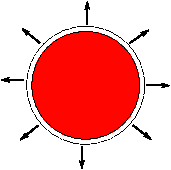
\includegraphics[width=\textwidth]{figs/pellet_exp.pdf}
        \caption{Fuel pellet}
    \end{subfigure}
    \hspace{6em}
    \begin{subfigure}[b]{0.25\textwidth}
        \centering
        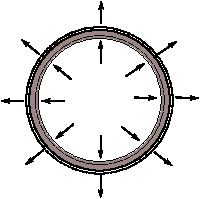
\includegraphics[width=\textwidth]{figs/clad_exp.pdf}
        \caption{Cladding}
    \end{subfigure}
    \caption{The radial expansion of fuel pellet and cladding.}
       \label{fig_31}
\end{figure}

\subsection{Calculation Flow} \label{sec34}

Figure \ref{fig_32} is a flow chart illustrating the calculation of geometrical changes due to thermal expansion. Initially, after several cycles of neutron tracking, the thermal-hydraulic (TH) solver is executed to determine the temperature distribution. This temperature distribution is then used to calculate pin-averaged fuel pellet and cladding temperatures, which are subsequently utilized to determine the corresponding expansion-induced geometrical changes in fuel pellets and cladding. Similarly, assembly-averaged temperatures are used to compute the geometrical changes in pin-pitch. Following this, core-averaged temperatures are used to thermally expand the assembly pitches uniformly. Finally, the material densities are updated to ensure the preservation of material mass throughout the process. These steps are repeated iteratively until all cycles are completed.

Once the geometrical changes due to thermal expansion are calculated during the TH update, this information is used to thermally expand the core geometry on-the-fly during subsequent cycles of neutron tracking. When a neutron is located in a pin cell after performing a random walk, MCS checks whether it originated from another pin cell or from the same one. If it originated from another pin cell, the fuel pellet and cladding surfaces in that pin cell are expanded based on the previously calculated geometrical changes. Additionally, if the neutron came from another assembly, the pin pitches within that assembly are uniformly expanded as well. These steps are summarized in Figure \ref{fig_33}.

\begin{figure}
    \centering
    \begin{minipage}{.32\textwidth}
      \centering
      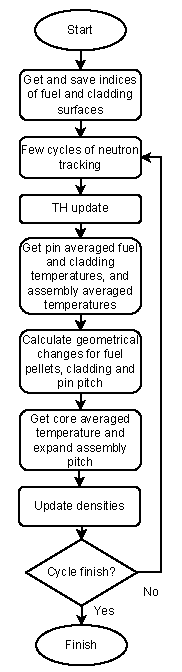
\includegraphics[width=\textwidth]{figs/te_calc_flow_1.pdf}
      \captionof{figure}{Calculation of geometrical changes due to thermal expansion.}
      \label{fig_32}
    \end{minipage}%
    \hspace{8em}
    \begin{minipage}{.34\textwidth}
      \centering
      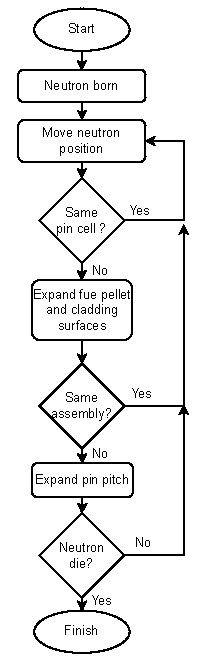
\includegraphics[width=\textwidth]{figs/te_calc_flow_2.pdf}
      \captionof{figure}{On-the-fly thermal expansion during neutron tracking.}
      \label{fig_33}
    \end{minipage}
\end{figure}
